\chapter{The SPICE Netlist Syntax}
\label{chap:spicecode}

This chapter presents the netlist syntax, which we plan to support in the NextGen SPICE library for importing circuits and in the standalone console application. The syntax presented here is a subset of that supported by SPICE3, and can be further restricted to that of SPICE2.

\section{General Syntax}
\label{chap:spicecode:general}
The SPICE netlist syntax is case insensitive. A netlist file consists of individual statements, which are separated by line breaks. If a statement is to span multiple lines, every subsequent line must be prefixed with a + symbol. The following code fragments are therefore equivalent. 

\begin{code}
V1 0 1
+ SIN 0 5V 10KHZ
\end{code}

\begin{code}
V1 0 1 SIN 0 5V 10KHZ
\end{code}

Statements themselves are made up of individual data fields, delimited by blank characters. The meaning of data fields depends on the actual statement and on the position inside the statement. Generally, a data field specifies either a name, or a numeric value, and is then called a name field or a number field, respectively.

\subsection{Number Fields}
\label{chap:spicecode:numfield}
If the statement expects a data field to represent a numeric value, then the (number) field should start with a digit. However, if a decimal number is specified, the leading zeros may be omitted (therefore, \texttt{.05} is a valid number field having the same value as \texttt{0.05}). It is also possible to specify the scale by either using suffixes like \texttt{E-9} or one of the scaling factors listed in the following table.

\begin{center}
\begin{tabular}{|l|l|}	
	\hline
	Factor & Scale \\
	\hline \hline
	T & $ 10^{12} $ \\ \hline
	G & $10^9$ \\ \hline
	MEG & $ 10^6 $ \\ \hline
	K & $ 10^3 $ \\ \hline
	M & $ 10^{-3} $ \\ \hline
	U & $ 10^{-6} $ \\ \hline
	N & $ 10^{-9} $ \\ \hline
	P & $ 10^{-12} $ \\ \hline
	F & $ 10^{-15} $ \\
	\hline
\end{tabular}
\end{center}

Any additional characters that follow the number and scale factor are ignored, so the fields \texttt{10000}, \texttt{10E+3V}, \texttt{10K}, \texttt{10KV}, \texttt{10KVOLTS} and \texttt{10KHz} all represent the same value. This is convenient, because the ignored part may be used to specify units and thus improve readability of the netlist file.

\subsection{Name Fields}

On the other hand, if a data field is to represent a name, an arbitrary string of alphanumeric characters can be used.

\subsection{Comments}
The input file can also contain comments, which are completely ignored by the parser. Comments begin with an asterisk * symbol, and end by a line break. Comments can be used to further improve readability of the netlist file.

\begin{code}
V1 0 in 5 		* a 5V voltage source between the ground and 'in' node
\end{code}

\section{Data Statements}
\label{chap:spicecode-devices}

Data statements are used to describe the actual circuit and can be further divided into \textit{device statements} and \textit{model statements}. Device statements specify individual circuit devices and their connections to circuit nodes and generally have the following form:

\begin{code}
<device name> <terminal connections> <device arguments>
\end{code}

The concrete SPICE device type is determined by the first letter of the device name, and from the device type, the number of terminal connections and arguments is derived. Like SPICE3, we will not pose any restrictions on the length of the device name.\footnote{in SPICE2, the length was limited to seven characters only}

After the name follows a list of nodes to which the device connects. Nodes are identified by arbitrary alphanumeric strings.\footnote{In SPICE2, nodes are identified by integers, one consequence of this is that \texttt{00} and \texttt{0} are equivalent in SPICE2, but not in SPICE3.} The ground node is identified as \texttt{0}. After the terminal connections follows a device dependent argument list.

Model statements are used to specify parameters for more complex semiconductor devices, so that multiple devices can have the same parameters without their extensive repetition throughout the netlist file. A model statement has the following structure:

\begin{code}
.MODEL <model name> <model type> (<model parameter list>) 
\end{code}

Each device can accept only model types corresponding to that particular device type. Each model type has a set of parameters, which are set in the model parameter list, each having its default value. When defining a new model, only non-default values need to be specified by a list of key value pairs in the form \texttt{<name>=<value>}. The model name is then supplied as an argument to semiconductor devices such as a diode. 

The following sections describe the formats of several SPICE device statements. Values beginning with N are for node connections, values enclosed in square brackets are optional. Also, when applicable, the available model types and names of their parameters are listed.

\subsection{Resistor}

\begin{circuitdev}
	(0,0) node[label=N+]{} to[R, *-*] (2,0) node[label=N-]{}
\end{circuitdev}

\begin{code}
R<name> N+ N- <resistance>
\end{code}

A simple ideal resistor device. The order of N+ and N- nodes has no effect on the circuit behavior.

Examples: 

\begin{code}
R1 1 2 5OHM
R2 2 3 1K
\end{code}

\subsection{Capacitor}

\begin{circuitdev}
	(0,0) node[label=N+]{} to[C, *-*] (2,0) node[label=N-]{}
\end{circuitdev}

\begin{code}
C<name> N+ N- <capacitance> [IC=<initial voltage>]
\end{code}

An ideal capacitor device, an initial voltage can be specified to set a specific condition at the beginning of the simulation. If an initial condition is not present, the capacitor is modeled as an open circuit in the first DC operating point calculation.

Examples: 

\begin{code}
C1 1 2 1F
C2 2 3 1N IC=1M
\end{code}

\subsection{Inductor}

\begin{circuitdev}
	(0,0) node[label=N+]{} to[L, *-*] (2,0) node[label=N-]{}
\end{circuitdev}

\begin{code}
L<name> N+ N- <capacitance> [IC=<initial current>]
\end{code}

An ideal inductor device, an initial current can be specified to set a specific condition at the beginning of the simulation. If an initial condition is not present, the inductor is modeled as an ideal short circuit in the first DC operating point calculation.

Examples: 

\begin{code}
L1 1 2 1F
L2 2 3 1N IC=1M
\end{code}

\subsection{Input sources}
\label{chap:spicecode-input-sources}

\begin{circuitdev}
	(0,0) node[label=N+]{} to[V, *-*] (2,0) node[label=N-]{}
	(4,0) node[label=N+]{} to[I, *-*] (6,0) node[label=N-]{}
\end{circuitdev}

\begin{code}
V<name> N+ N- <source function>
I<name> N+ N- <source function>
\end{code}

NextGen SPICE supports complex specification of input source behaviors. Possible source functions are listed below.

\subsubsection{DC Source}
\begin{code}
[DC] <voltage>
\end{code}

A source that has a constant value, the \texttt{DC} identifier can be omitted.

Examples:

\begin{code}
V1 1 0 5V
I2 1 2 DC 10KV
\end{code}

\subsubsection{Sinusoidal Source}

\begin{code}
SIN <vo> <va> <freq> [<td> [<th> [<ph>]]]
\end{code}

\begin{center}
\begin{tabular}{|l|l|}
	\hline
Parameter & Meaning \\ \hline \hline
\texttt{<vo>} & Value offset \\ \hline
\texttt{<va>} & Value amplitude \\ \hline
\texttt{<fr>} & Waveform frequency \\ \hline
\texttt{<td>} & Delay time \\ \hline
\texttt{<th>} & Damping factor \\ \hline
\texttt{<phase>} & Phase offset \\ \hline
\end{tabular}
\end{center}

A sinusoidal source with amplitude damping. The value of the source function is given by

\[f(t) = \begin{cases}

\texttt{<vo> } & \text{if } t < \texttt{<td>} \\
\texttt{<vo>} + \texttt{<va>} \begin{aligned}
&\cdot e^{- (t - \texttt{<td>}) \cdot \texttt{<th>}}\\
&\cdot \sin{(2 \pi \cdot  (\texttt{<fr>} \cdot (t - \texttt{<td>}) + \texttt{<ph>}))}
\end{aligned}  & \text{if } t \ge \texttt{<td>}
\end{cases}\] 


Example:

\begin{code}
V1 1 0 SIN 1 5 2KHZ 1MS 0.5K
\end{code}

\begin{center}
	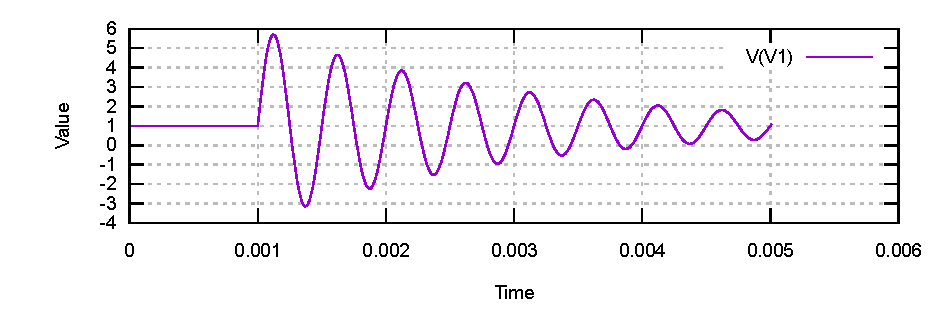
\includegraphics[width=0.85\linewidth]{source-sin}
\end{center}

\pagebreak
\subsubsection{Exponential Source}

\begin{code}
EXP <v1> <v2> [<td1> <tau1> [<td2> <tau2>]]
\end{code}

\begin{center}
	\begin{tabular}{|l|l|}
		\hline
		Parameter & Meaning \\ \hline \hline
		\texttt{<v1>} & Initial value \\ \hline
		\texttt{<v2>} & Pulse value \\ \hline
		\texttt{<td1>} & Delay before first e.g.\ \\ \hline
		\texttt{<tau1>} & First e.g.\ time constant \\ \hline
		\texttt{<td2>} & Delay before second e.g.\ \\ \hline
		\texttt{<tau2>} & Second e.g.\ time constant \\ \hline
	\end{tabular}
\end{center}

A pulsing source with exponential rising and falling edges. Values of the source are given by:

\[
f(t) = \begin{cases}
\texttt{<v1>} & \text{if } t < \texttt{<td1>} \\\\
\texttt{<v1>} + \left( \texttt{<v1>} - \texttt{<v2>} \left[1-e^{\frac{-(t-\texttt{<td1>})}{\texttt{<tau1>}}}\right] \right)& \text{if } \texttt{<td1>} \ge t > \texttt{<td2>} \\\\
\texttt{<v1>} \begin{aligned}
&+ \left( \texttt{<v1>} - \texttt{<v2>} \left[1-e^{\frac{-(t-\texttt{<td1>})}{\texttt{<tau1>}}}\right] \right) \\
&+ \left( \texttt{<v2>} - \texttt{<v1>} \left[1-e^{\frac{-(t-\texttt{<td2>})}{\texttt{<tau2>}}}\right] \right)
\end{aligned}& \text{if } t \ge \texttt{<td2>} \\
\end{cases}
\]

Example:

\begin{code}
V1 1 0 EXP 1 5 1MS 0.5M 4MS 0.1M 
\end{code}

\begin{center}
	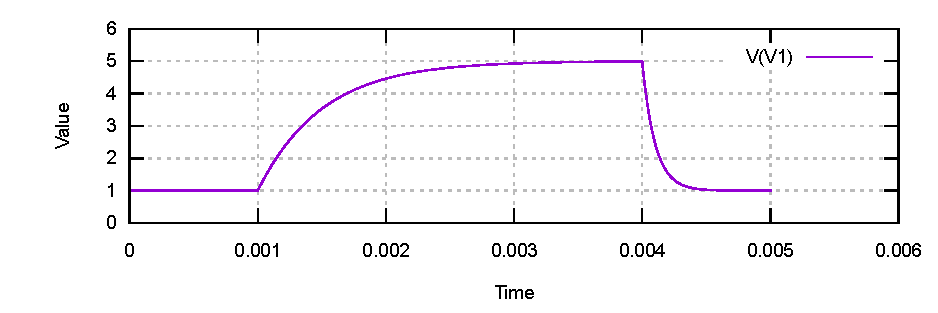
\includegraphics[width=0.85\linewidth]{source-exp}
\end{center}

\subsubsection{Pulse Source}

\begin{code}
PULSE <v1> <v2> <td> <tr> <tf> <ton> <period>
\end{code}

\begin{center}
	\begin{tabular}{|l|l|}
		\hline
		Parameter & Meaning \\ \hline \hline
		\texttt{<v1>} & Initial value \\ \hline
		\texttt{<v2>} & Pulse value \\ \hline
		\texttt{<td>} & Delay before rising e.g.\ of the pulse \\ \hline
		\texttt{<tr>} & Time of the rising e.g.\ of the pulse\\ \hline
		\texttt{<tf>} & Time of the falling e.g.\ of the pulse \\ \hline
		\texttt{<ton>} & Duration of the pulse \\ \hline
		\texttt{<period>} & Period of the source \\ \hline
	\end{tabular}
\end{center}

A source that sends individual pulses.

Example:

\begin{code}
V1 1 0 PULSE 1 5 1MS 0.5MS 1.5MS 1MS 5MS
\end{code}

\begin{center}
	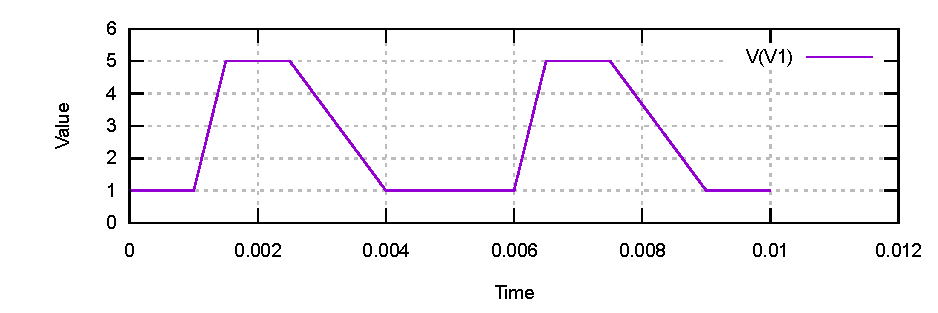
\includegraphics[width=0.85\linewidth]{source-pulse}
\end{center}

\subsubsection{Piecewise Linear Source}

\begin{code}
PWL <t1> <v1> [<t2> <v2> [<t3> <v3> [...]]]
\end{code}

An arbitrary piece-wise linear source. The argument list consists of pairs of timepoints and source values. The intermediate values are determined using linear interpolation.

Example:
\begin{code}
V1 1 0 PWL 0MS 1 1MS 2 3MS -1 3.1MS 0 5MS 1
\end{code}

\begin{center}
	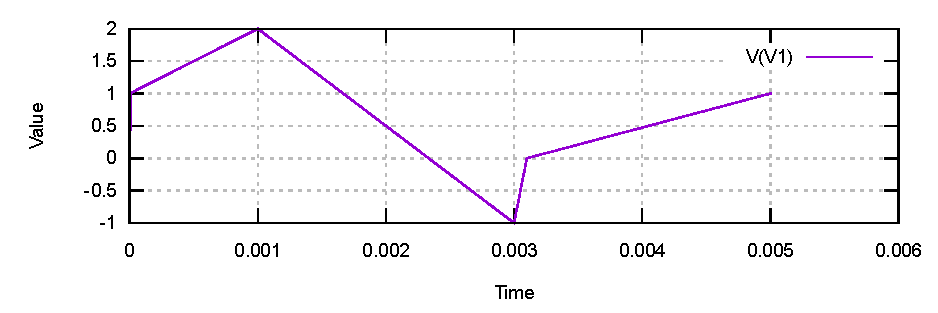
\includegraphics[width=0.85\linewidth]{source-pwl}
\end{center}

\subsubsection{AM Source}
\begin{code}
AM <amp> <dc> <fm> <fc> [<td> [<ph>]]
\end{code}

\begin{center}
	\begin{tabular}{|l|l|}
		\hline
		Parameter & Meaning \\ \hline \hline
		\texttt{<amp>} & Peak amplitude of the unmodulated signal. \\ \hline
		\texttt{<dc>} & DC offset \\ \hline
		\texttt{<fm>} & Modulation frequency \\ \hline
		\texttt{<fc>} & Carrier frequency \\ \hline
		\texttt{<td>} & Delay before the signal \\ \hline
		\texttt{<ph>} & Phase offset \\ \hline
	\end{tabular}
\end{center}

% arbitrary page break to better accmodate the pictures
\pagebreak
A source with an amplitude modulated signal. The value at any given timepoint is given by

\[
f(t) = \texttt{<amp>} \begin{aligned}
&\cdot \left( \texttt{<dc>}  + \sin{
	\left(
	2\pi \cdot \texttt{<fm>} \cdot  \left(t - \texttt{<td>}\right)
	\right)} + \texttt{<ph>} \right) 
\\
&\cdot \sin{
	\left(
	2\pi \cdot \texttt{<fc>} \cdot  \left(t - \texttt{<td>} \right) + \texttt{<ph>}
	\right)}.
\end{aligned} 
\]

Example:

\begin{code}
V1 1 0 AM 5 2 0.5KHZ 4KHZ 2MS
\end{code}

\begin{center}
	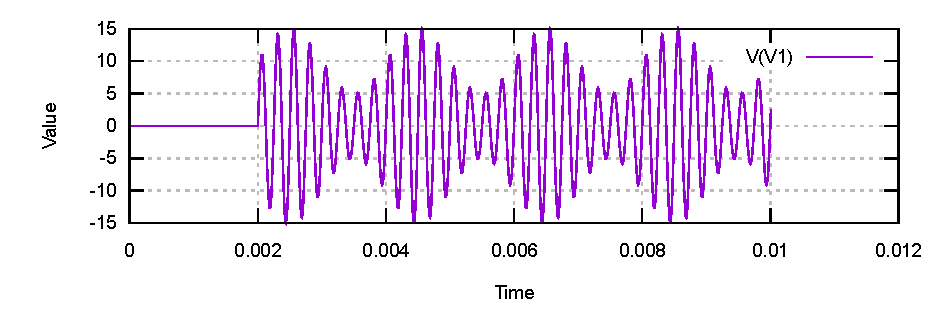
\includegraphics[width=0.85\linewidth]{source-am}
\end{center}

\subsubsection*{SFFM Source}
\begin{code}
SFFM <dc> <amp> <fc> <m> <fm>
\end{code}

\begin{center}
	\begin{tabular}{|l|l|}
		\hline
		Parameter & Meaning \\ \hline \hline
		\texttt{<dc>} & DC offset of the signal \\ \hline
		\texttt{<amp>} & Amplitude of the carrier. \\ \hline
		\texttt{<fc>} & Carrier frequency \\ \hline
		\texttt{<m>} & Modulation index \\ \hline
		\texttt{<fm>} & Modulation frequency \\ \hline
	\end{tabular}
\end{center}

A source with a frequency modulated signal. The value at any given timepoint is given by

\[
f(t) = \texttt{<dc>} + \texttt{<amp>} \cdot \sin{
	\left(
	2\pi \cdot \texttt{<fc>} \cdot  \left(t - \texttt{<td>}\right) + m \cdot \sin{
		\left(
		2\pi \cdot \texttt{<fm>} \cdot  \left(t - \texttt{<td>}\right)
		\right)}
	\right)}.
\]

Example:

\begin{code}
V1 1 0 SFFM 2 1 1KHZ 3 0.2KHZ 
\end{code}

\begin{center}
	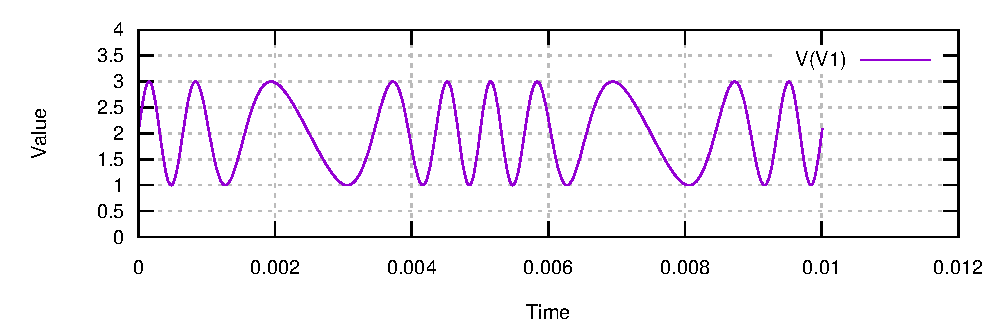
\includegraphics[width=0.85\linewidth]{source-sffm}
\end{center}


\subsection{Controlled Sources}

SPICE supports linear dependent sources, both current and voltage controlled. In the case of voltage controlled sources, an additional pair of terminals is specified, and the value of the source is linearly dependent on the voltage between those control terminals. In case of current controlled sources, the name of a voltage source is supplied and the value of the source depends linearly on the current flowing through said device.\footnote{The reason that only voltage source can be used is that the current flowing through the voltage source is directly accessible through a circuit variable in the equation system. Also, because earlier versions of SPICE could output only currents flowing through voltage sources, it became a standard practice to use 0V voltage sources as amperemeters.} The coefficient of linear dependence, called the \textit{gain} is supplied as the last parameter.

\subsubsection{Voltage Controlled Voltage Source}
\begin{circuitdev}
	(0,0) node[circ,label=NC+]{} 
	-- (1,0)
	-- (1,-2)
	-- (0,-2) node[circ,label=NC-]{}
	
	(3,0) node[circ,label=N+]{}
	-- (2,0)
	to[V] (2, -2)
	-- (3,-2) node[circ,label=N-]{}
\end{circuitdev}
\begin{code}
E<name> N+ N- NC+ NC- <gain>
\end{code}



Example: 

\begin{code}
E1 1 2 3 4 100
\end{code}


\subsubsection{Voltage Controlled Current Source}
\begin{circuitdev}
	(0,0) node[circ,label=NC+]{} 
	-- (1,0)
	-- (1,-2)
	-- (0,-2) node[circ,label=NC-]{}
	
	(3,0) node[circ,label=N+]{}
	-- (2,0)
	to[I] (2, -2)
	-- (3,-2) node[circ,label=N-]{}
\end{circuitdev}
\begin{code}
G<name> N+ N- NC+ NC- <gain>
\end{code}

Example: 

\begin{code}
G1 1 2 3 4 100
\end{code}


\subsubsection{Current Controlled Voltage Source}
\begin{circuitdev}
	(0,0) 
	-- (1,0)
	to[V,a=vsource] (1,-2)
	-- (0,-2)
	
	(4,0) node[circ,label=N+]{}
	-- (3,0)
	to[cV] (3, -2)
	-- (4,-2) node[circ,label=N-]{}
\end{circuitdev}
\begin{code}
H<name> N+ N- <vsource> <gain>
\end{code}

Example: 

\begin{code}
VMETER 1 2 0
H1 2 3 VMETER
\end{code}

\subsubsection{Current Controlled Current Source}
\begin{circuitdev}
	(0,0) 
	-- (1,0)
	to[V,a=vsource] (1,-2)
	-- (0,-2)
	
	(4,0) node[circ,label=N+]{}
	-- (3,0)
	to[cI] (3, -2)
	-- (4,-2) node[circ,label=N-]{}
\end{circuitdev}
\begin{code}
F<name> N+ N- <vsource> <gain>
\end{code}

Example: 

\begin{code}
VMETER 1 2 0
F1 2 3 VMETER
\end{code}

\subsection{Diode}
\begin{circuitdev}
	(0,0) node[label=N+]{} to[D, *-*] (2,0) node[label=N-]{}
\end{circuitdev}

\begin{code}
D<name> N+ N- <model name>
\end{code}

A semiconductor diode device. The physical parameters of a diode are set using a \texttt{.MODEL} statement with the \texttt{D} model type. The following table lists supported model parameters for the diode model. The parameters in gray are parsed, but do not affect the simulation in the current implementation.

\begin{center}
	\begin{tabu}{|l|l|r l|}
		\hline
		Parameter name & Description & \multicolumn{2}{l|}{Default value} \\ 
		\hline \hline
		IS & Saturation current & $ 1 \cdot 10^{-14}$& A  \\ \hline	
		RS & Ohmic resistance & $ 0 $& \\ \hline		
		N & Emission coefficient & $ 1 $& \\ \hline	
		TT & Transit-time current & $ 0$& s \\ \hline	
		CJO & Zero-bias junction capacitance & $ 0$& F \\ \hline	
		VJ & Junction potential & $ 1$& V \\ \hline	
		M & Grading coefficient & $ 0.5 $& \\ \hline	
		\rowfont{\color{lightgray}}	EG & Activation ene.g.\ & $ 1.11$& eV\\ \hline	
		\rowfont{\color{lightgray}}	XTI & Saturation-current temperature exponent & $ 3 $& \\ \hline	
		\rowfont{\color{lightgray}}	KF & Flicker noise coefficient & $ 0 $& \\ \hline	
		\rowfont{\color{lightgray}}	AF & Flicker noise exponent & $ 1 $& \\ \hline	
		\rowfont{\color{lightgray}}	FC & \makecell[l]{Coefficient for forward-bias \\
			 depletion capacitance formula} & $ 0.5 $&\\ \hline	
		BV & Reverse breakdown voltage & $ \infty{}$& V \\ \hline	
		\rowfont{\color{lightgray}}	IBV & Current at breakdown voltage & $ 1 \cdot 10^{-3}$& A \\ \hline	
		TNOM & Parameter measurement temperature & $ 27$& °C \\ \hline	
	\end{tabu}
\end{center}

Example:
\begin{code}
D1 1 2 1N4148
.MODEL 1N4148 D(IS=2.52N RS=.568 N=1.752 CJO=4P M=.4 TT=20N VJ=20 BV=75)
\end{code}

\subsection{BJT Transistor}
\begin{circuitdev}
(0,0) node[npn](npn1) {}
(npn1.base) node[circ, label=180:NB] {}
(npn1.collector) node[circ, label=NC] {}
(npn1.emitter) node[circ, label=270:NE] {}

(4,0) node[pnp,yscale=-1](pnp1) {}
(pnp1.base) node[circ, label=180:NB] {}
(pnp1.collector) node[circ, label=NC] {}
(pnp1.emitter) node[circ, label=270:NE] {};
\end{circuitdev}

\begin{code}
Q<name> NC NB NE <model name>
\end{code}

A semiconductor BJT transistor device. The physical parameters of a BJT are set using a \texttt{.MODEL} statement, as well as the polarity of the transistor. There are two model types for a BJT transistor: \texttt{NPN} and \texttt{PNP}. Both model types accept the same parameters, which are listed in the following table. The parameters in gray are parsed, but do not affect the simulation in the current implementation.

\begin{center}
	\begin{longtable}{|l|l|r l|}
		\hline
		\makecell[l]{Parameter \\ name} & Description & \multicolumn{2}{l|}{Default value} \\ 
		\hline \hline
		IS 	&	Transport saturation current	&	1.0e16 &	A 	 \\ \hline
BF 	&	Ideal maximum forward beta	&	100 &	 	 \\ \hline
NF 	&	Forward current emission coefficient	&	1.0 	   &	 	 \\ \hline
VAF 	&	Forward Early voltage	&	$ \infty{}$    &	V 	 \\ \hline
IKF 	&	Corner for forward beta high current roll-off	&	$ \infty{}$    &	A 	 \\ \hline
ISE 	&	B-E leakage saturation current	&	0 	&   	A 	 \\ \hline
NE 	&	B-E leakage emission coefficient	&	1.5 	&   	 	 \\ \hline
BR 	&	Ideal maximum reverse beta 	&	1 	&   	 	 \\ \hline
NR 	&	Reverse current emission coefficient	&	1 	&   	 	 \\ \hline
VAR 	&	Reverse Early voltage	&	$ \infty{}$    &	V 	 \\ \hline
IKR 	&	Corner for reverse beta high current roll-off	&	$ \infty{}$    &	A 	 \\ \hline
ISC 	&	Leakage saturation current	&	0 	&   	A 	 \\ \hline
NC 	&	Leakage emission coefficient	&	2 	&   	 	 \\ \hline
	RB 	&		Zero bias base resistance	&		0 	&	   	 	 \\ \hline
\color{lightgray}	IRB 	&	\color{lightgray}	\makecell[l]{Current where base resistance \\ falls halfway to its min value}	&	\color{lightgray}	$ \infty{}$ &	\color{lightgray}	A 	 \\ \hline
\color{lightgray}	RBM 	&	\color{lightgray}	Minimum base resistance at high currents	&	\color{lightgray}	RB  &	\color{lightgray}	 	 \\ \hline
RE 	&		Emitter resistance	&		0 	&	   	 	 \\ \hline
RC 	&		Collector resistance 	&		0 	&	   	 	 \\ \hline
CJE 	&		B-E zero-bias depletion capacitance	&		0 	&	   	F 	 \\ \hline
VJE 	&		B-E built-in potential	&		0.75    &		V 	 \\ \hline
MJE 	&		B-E junction exponential factor 	&		0.33    &		 	 \\ \hline
TF 	&		Ideal forward transit time 	&		0 	&	   	s 	 \\ \hline
\color{lightgray}	XTF	&	\color{lightgray}	Coefficient for bias dependence of TF 	&	\color{lightgray}	0 	&	\color{lightgray}   	 	 \\ \hline
\color{lightgray}	VTF 	&	\color{lightgray}	Voltage describing VBC dependence of TF 	&	\color{lightgray}	$ \infty{}$    &	\color{lightgray}	V 	 \\ \hline
\color{lightgray}	ITF 	&	\color{lightgray}	High-current parameter  for effect on TF 	&	\color{lightgray}	0 	&	\color{lightgray}   	A 	 \\ \hline
\color{lightgray}	PTF 	&	\color{lightgray}	Excess phase at freq=1.0/(TF*2PI) Hz 	&	\color{lightgray}	0 	&	\color{lightgray}   	deg 	 \\ \hline
CJC 	&		B-C zero-bias depletion capacitance 	&		0 	&	   	F 	 \\ \hline
VJC 	&		B-C built-in potential 	&		0.75    &		V 	 \\ \hline
MJC 	&		B-C junction exponential factor 	&		0.33    &		 	 \\ \hline
\color{lightgray}	XCJC 	&	\color{lightgray}	\makecell[l]{Fraction of B-C depletion capacitance \\ connected to internal base node} 	&	\color{lightgray}	1 	&	\color{lightgray}   	 	 \\ \hline
TR 	&		Ideal reverse transit time 	&		0 	&	   	s 	 \\ \hline
CJS 	&		Zero-bias collector-substrate capacitance 	&		0 	&	   	F 	 \\ \hline
VJS 	&		Substrate junction built-in potential 	&		0.75    &		V 	 \\ \hline
MJS 	&		Substrate junction exponential factor 	&		0 	&	   	 	 \\ \hline
\color{lightgray}	XTB 	&	\color{lightgray}	Forward and reverse beta  temperature exponent 	&	\color{lightgray}	0 	&	\color{lightgray}   	 	 \\ \hline
\color{lightgray}	EG	&	\color{lightgray}	Ene.g.\ gap for temperature  effect on IS 	&	\color{lightgray}	1.11    &	\color{lightgray}	eV 	 \\ \hline
\color{lightgray}	XTI	&	\color{lightgray}	Temperature exponent for effect on IS 	&	\color{lightgray}	3 	&	\color{lightgray}   	 	 \\ \hline
\color{lightgray}	KF 	&	\color{lightgray}	Flicker-noise coefficient 	&	\color{lightgray}	0 	&	\color{lightgray}   	 	 \\ \hline
\color{lightgray}	AF 	&	\color{lightgray}	Flicker-noise exponent 	&	\color{lightgray}	1 	&	\color{lightgray}   	 	 \\ \hline
FC 	&		\makecell[l]{Coefficient for forward-bias \\ depletion capacitance formula} 	&		0.5 	&	   	 	 \\ \hline

TNOM 	&	Parameter measurement temperature 	&	27  &	°C 	 \\ \hline


	\end{longtable}
\end{center}

Examples:

\begin{code}
Q1 1 2 3 QMOD1
.MODEL QMOD1 PNP(IS=1P)

Q2 4 5 6 QNL
.MODEL QNL NPN(BF=80 RB=100 TF=0.3NS TR=6NS CJE=3PF CJC=2PF VAF=50V)
\end{code}

\subsection{Subcircuits}
\label{chap:spicecode:subcircuits}
Subcircuits are a SPICE netlist term for device macromodels mentioned back in the introduction chapter. The following syntax is used.

\begin{code}
.SUBCKT <subcircuit name> <terminal nodes>
<subcircuit description>
.ENDS
\end{code}

The description of the subcircuit has to be enclosed between \texttt{.SUBCKT} and \texttt{.ENDS} statements. The \texttt{.SUBCKT} statement states the name of the subcircuit and lists the names of terminal nodes, which will then be used to connect the subcircuit to the outer circuit. There must be at lesat one terminal node and none of them can be 0 (the ground node).

The actual description of the subcircuit can contain only data statements -- device statements, \texttt{.MODEL} statements, and other \texttt{.SUBCKT} statements. Also, it is customary to place a comment line describing the meaning of the terminal nodes (like in figure~\ref{fig:example_subcircuit}).

Any names defined inside a subcircuit are strictly local to the subcircuit. Therefore, models and subcircuits defined inside the subcircuit cannot be used after the \texttt{.ENDS} statement.

A subcircuit can then be used as an individual device by the following syntax:

\begin{code}
X<name> <terminal nodes> <subcircuit name>
\end{code}

where \texttt{<subcircuit name>} is the name supplied in the corresponding \texttt{.SUBCKT} statement, and \texttt{<terminal nodes>} names the appropriate number of nodes to which the subcircuit should connect.

Example:
\begin{code}
.SUBCKT ACAMPLIFIER 2 1 3
R1 1 4 2K
R2 4 0 500
C1 2 4 10n
Q1 3 4 5 2N2222
Rc 1 3 2K
Re 5 0 1e3
.MODEL 2N2222 PNP(BF=50 IS=1E-13 VBF=50)
.ENDS

XOPAMP 1 2 3 ACAMPLIFIER
\end{code}

\subsection{Summary of the Device Statements}

\begin{center}
	\begin{tabular}{|l|l|}
		\hline
		Device & Syntax \\ 
		\hline \hline
		Resistor & \texttt{R<name> N+ N- <resistance>} \\ \hline
		Capacitor & \texttt{C<name> N+ N- <capacitance> [IC=<voltage>]} \\ \hline
		Inductor & \texttt{L<name> N+ N- <inductance> [IC=<current>]} \\ \hline
		Voltage source & \texttt{V<name> N+ N- <source function>} \\ \hline
		Current source & \texttt{I<name> N+ N- <source function>} \\ \hline
		\makecell[l]{Voltage controlled \\ voltage source} & \texttt{E<name> N+ N- NC+ NC- <gain>} \\ \hline
		\makecell[l]{Voltage controlled \\ current source} & \texttt{G<name> N+ N- NC+ NC- <gain>} \\ \hline
		\makecell[l]{Current controlled \\ voltage source} & \texttt{H<name> N+ N- <voltage source> <gain>} \\ \hline
		\makecell[l]{Current controlled \\ current source} & \texttt{F<name> N+ N- <voltage source> <gain>} \\ \hline
		Diode & \texttt{D<name> N+ N- <model name>} \\ \hline
		BJT transistor & \texttt{Q<name> NC NB NE <model name>} \\ \hline
	\end{tabular}
\end{center}

\newpage
\section{Control Statements}

Control statements are used for performing circuit simulations.

\subsection{.OP Statement}

\begin{code}
.OP
\end{code}

The \texttt{.OP} statement is used for requesting DC operating point analysis, which means calculating the values of node voltages and branch currents corresponding to a stable state of the circuit. This statement does not have any arguments.

\subsection{.TRAN Statement}

\begin{code}
.TRAN <timestep> <stop time> [<start time>]
\end{code}

This statement is used for requesting transient analysis --- time-domain simulation of the circuit --- for the specified duration with the given timestep. For each timepoint, an operating point is established, and time-dependent behavior of devices such as capacitor and inductor is modelled using numerical integration methods. If we are interested only in data after a certain timepoint, we can use the third optional parameter to instruct the simulator to not print simulation results until a certain timepoint.

\section{Output Statements}
\label{chap:spicecode-output}

Output statements can be used to select which data should be printed in the simulator's output. If no output statement is provided, NextGen SPICE will print all available data. Currently, the only supported statement is the \texttt{.PRINT} statement.

\begin{code}
.PRINT <analysis type> <list of requested data>
\end{code}

The analysis type is either \texttt{OP} or \texttt{TRAN}, indicating from which analysis type the data are requested. Following table summarizes the possible data specifiers.

\begin{center}
	\begin{tabular}{|l|l|}
		\hline
		Specifier & Description \\ \hline \hline
		\texttt{V(<node>)} & Voltage of the node \texttt{<node>} \\ \hline
		\texttt{V(<node1>,<node2>)} & Voltage between nodes \texttt{<node1>} and \texttt{<node2>} \\ \hline
		\texttt{V(<device>)} & Voltage across the \texttt{<device>} device\footnotemark  \\ \hline
		\texttt{I(<device>)} & Current flowing through the \texttt{<device>} device$^{\ref{footnote:spice_print}}$. \\ \hline
	\end{tabular}
\end{center}

\footnotetext{\label{footnote:spice_print}Only devices having exactly two terminals are allowed.}


\section{Netlist File Structure}
The structure of a netlist can be almost arbitrary, the only restrictions are that the first line, called the \textit{title line}, should contain a brief description of the netlist contents (and is not interpreted as a statement), and that the last statement is an \texttt{.END} statement. There are no restrictions on the relative order of statements in the netlist. For example, semiconductor device models can be used in device statements even before they are defined by their respective \texttt{.MODEL} statement. However, even though any order is possible, netlist files are commonly structured in the following manner:

\begin{itemize}
	\item Title
	\item Device statements
	\item \texttt{.MODEL} statements
	\item Control statements
	\item Output statements
	\item \texttt{.END} statement
\end{itemize}

\section{Circuit Topology Constraints}
\label{chap:spicecode:topology}

There are some restrictions on how circuit devices can be connected to nodes. These restrictions help ensure that the equation system rising from the simulated circuit always has a unique solution. The rules are the following:

\begin{itemize}
	\item The circuit may not contain cycles consisting of voltage defined devices (e.g.\ voltage sources and inductors)
	\item The circuit may not contain cutsets consisting of current defined devices (e.g.\ current sources and capacitors)
	\item In a circuit, there must exist a path from each node to the ground node
	\item In a subcircuit, there must exist a path between each pair of terminals that does not contain the ground node 
\end{itemize}
